\documentclass[11pt, tikz]{standalone}
\usepackage[T1]{fontenc}
\usepackage[utf8]{inputenc}
%\usepackage{textcomp}
%\renewcommand{\ttdefault}{lmtt} % 
\usepackage{amsmath}
\usetikzlibrary{arrows.meta, decorations.pathmorphing, positioning, calc}
\usepackage{xcolor}

\begin{document}\sffamily
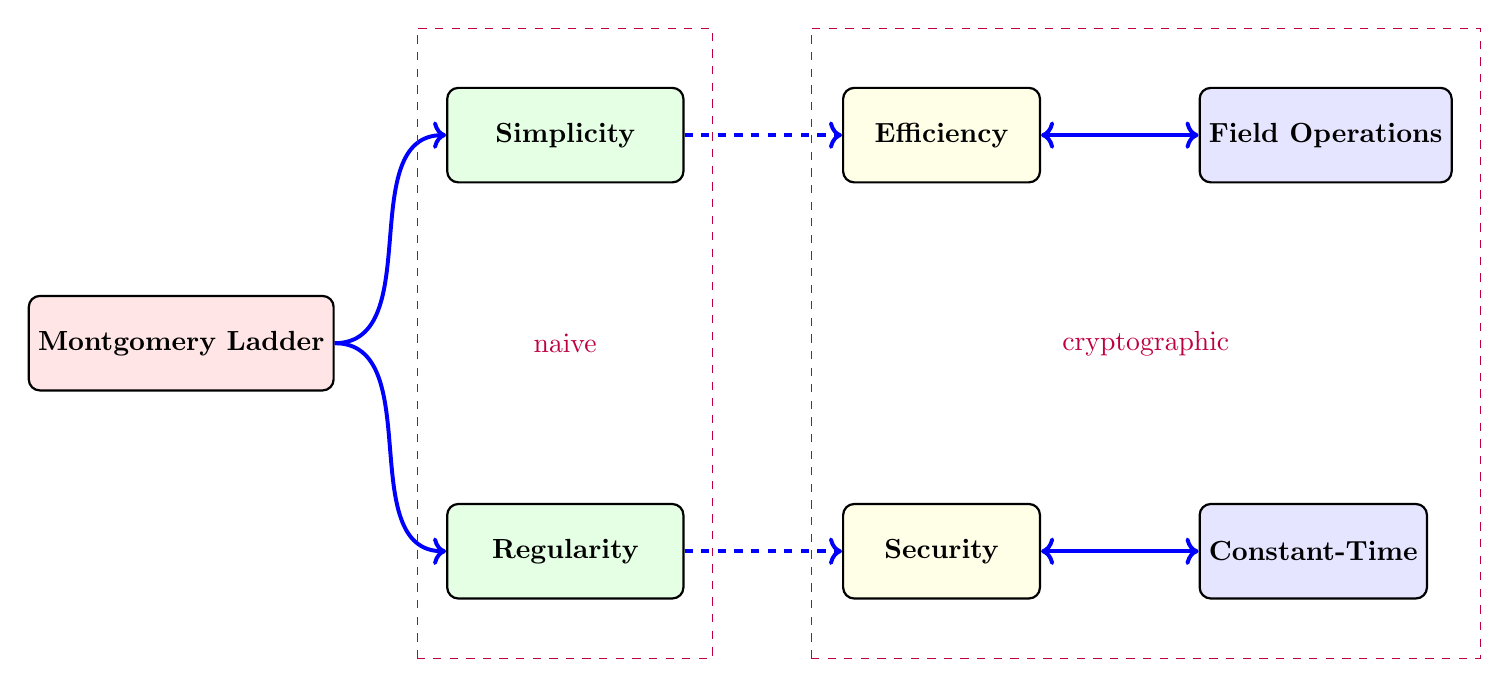
\begin{tikzpicture}[
	bluebox/.style={rectangle, draw, thick, rounded corners, minimum height=1.2cm, minimum width=2.5cm, align=center, fill=blue!10},
	yellowbox/.style={rectangle, draw, thick, rounded corners, minimum height=1.2cm, minimum width=2.5cm, align=center, fill=yellow!10},
	greenbox/.style={rectangle, draw, thick, rounded corners, minimum height=1.2cm, minimum width=3cm, align=center, fill=green!10},
	redbox/.style={rectangle, draw, thick, rounded corners, minimum height=1.2cm, minimum width=3cm, align=center, fill=red!10},
	arrow/.style={->, line width=.5mm},
	every node/.style={align=center}
	]
	\node[redbox] (mont) {\textbf{Montgomery Ladder}};
	\node[greenbox, above right=2cm of mont] (simple) {\bfseries Simplicity};
	\node[greenbox, below right=2cm of mont] (regular) {\bfseries Regularity};
	\node[yellowbox, right=2cm of simple] (efficiency) {\bfseries Efficiency};
	\node[yellowbox, right=2cm of regular] (security) {\bfseries Security};
	\node[bluebox, right=2cm of efficiency] (field) {\bfseries Field Operations};
	\node[bluebox, right=2cm of security] (constant) {\bfseries Constant-Time};
	\draw[arrow, blue, out=0, in=180] (mont) to (simple);
	\draw[arrow, blue, out=0, in=180] (mont) to (regular);
	\draw[dashed, arrow, blue, out=0, in=180] (simple) to (efficiency);
	\draw[dashed, arrow, blue, out=0, in=180] (regular) to (security);
	\draw[<->, line width=.5mm, blue, out=0, in=180] (efficiency) to (field);
	\draw[<->, line width=.5mm, blue, out=0, in=180] (security) to (constant);
	\draw[dashed, purple] (3,-4) rectangle (6.75,4) node[midway] {naive};
	\draw[dashed, purple] (8,-4) rectangle (16.5,4) node[midway] {cryptographic};
\end{tikzpicture}
\end{document}
